\documentclass{article}

\usepackage{fancyhdr}
\usepackage{extramarks}
\usepackage{amsmath}
\usepackage{amsthm}
\usepackage{amssymb}
\usepackage{amsfonts}
\usepackage{tikz}
\usepackage[plain]{algorithm}
\usepackage{algpseudocode}
\usepackage{mathpazo}
\usepackage{systeme}
\usepackage{multirow,array}
\usepackage{xcolor}
\usepackage{tikz-qtree}
\usepackage[long]{optidef}
\usepackage{tikz}
\usepackage{apacite}
\usepackage{mathtools}
\usepackage[english]{babel}
\usepackage[utf8x]{inputenc}
\usepackage{amssymb}
\usepackage{booktabs}
\usepackage{listings}
\usepackage{graphicx}
\usepackage{subcaption}

\newcommand{\R}{\mathbf{R}}  
\newcommand{\Z}{\mathbf{Z}}
\newcommand{\N}{\mathbf{N}}
\newcommand{\Q}{\mathbf{Q}}
\newcommand*{\QEDA}{\hfill\ensuremath{\blacksquare}}%

\tikzset{main node/.style={circle,draw,minimum size=1.5cm,inner sep=0pt},
            }


\usetikzlibrary{automata,positioning}

%
% Basic Document Settingshttps://www.overleaf.com/6212182343ggsvjzswgdnx
%

\topmargin=-0.45in
\evensidemargin=0in
\oddsidemargin=0in
\textwidth=6.5in
\textheight=9.0in
\headsep=0.25in

\linespread{1.1}

\pagestyle{fancy}
\chead{\hmwkTitle}
\rhead{\firstxmark}
\lfoot{\lastxmark}
\cfoot{\thepage}

\renewcommand\headrulewidth{0.4pt}
\renewcommand\footrulewidth{0.4pt}

\setlength\parindent{0pt}

%
% Create Problem Sections
%

\newcommand{\enterProblemHeader}[1]{
    \nobreak\extramarks{}{Problem \arabic{#1} continued on next page\ldots}\nobreak{}
    \nobreak\extramarks{Problem \arabic{#1} (continued)}{Problem \arabic{#1} continued on next page\ldots}\nobreak{}
}

\newcommand{\exitProblemHeader}[1]{
    \nobreak\extramarks{Problem \arabic{#1} (continued)}{Problem \arabic{#1} continued on next page\ldots}\nobreak{}
    \stepcounter{#1}
    \nobreak\extramarks{Problem \arabic{#1}}{}\nobreak{}
}

\DeclarePairedDelimiter\floor{\lfloor}{\rfloor}


\newenvironment{theorem}[2][Theorem]{\begin{trivlist}
\item[\hskip \labelsep {\bfseries #1}\hskip \labelsep {\bfseries #2.}]}{\end{trivlist}}
\newenvironment{lemma}[2][Lemma]{\begin{trivlist}
\item[\hskip \labelsep {\bfseries #1}\hskip \labelsep {\bfseries #2.}]}{\end{trivlist}}
\newenvironment{claim}[2][Claim]{\begin{trivlist}
\item[\hskip \labelsep {\bfseries #1}\hskip \labelsep {\bfseries #2.}]}{\end{trivlist}}
\newenvironment{problem}[2][Problem]{\begin{trivlist}
\item[\hskip \labelsep {\bfseries #1}\hskip \labelsep {\bfseries #2.}]}{\end{trivlist}}
\newenvironment{proposition}[2][Proposition]{\begin{trivlist}
\item[\hskip \labelsep {\bfseries #1}\hskip \labelsep {\bfseries #2.}]}{\end{trivlist}}
\newenvironment{corollary}[2][Corollary]{\begin{trivlist}
\item[\hskip \labelsep {\bfseries #1}\hskip \labelsep {\bfseries #2.}]}{\end{trivlist}}
\newcommand*\Eval[3]{\left.#1\right\rvert_{#2}^{#3}}
\newenvironment{solution}{\begin{proof}[Solution]}{\end{proof}}


\setcounter{secnumdepth}{0}
\newcounter{partCounter}
\newcounter{homeworkProblemCounter}
\setcounter{homeworkProblemCounter}{1}
\nobreak\extramarks{Problem \arabic{homeworkProblemCounter}}{}\nobreak{}

%
% Homework Problem Environment
%
% This environment takes an optional argument. When given, it will adjust the
% problem counter. This is useful for when the problems given for your
% assignment aren't sequential.
%
\newenvironment{homeworkProblem}[1][-1]{
    \ifnum#1>0
        \setcounter{homeworkProblemCounter}{#1}
    \fi
    \section{Problem \arabic{homeworkProblemCounter}}
    \setcounter{partCounter}{1}
    \enterProblemHeader{homeworkProblemCounter}
}{
    \exitProblemHeader{homeworkProblemCounter}
}

%
% Homework Details
%   - Title
%   - Due date
%   - Class
%   - Section/Time
%   - Instructor
%   - Author
%

\newcommand{\hmwkTitle}{Assignment 1\ }
\newcommand{\hmwkDueDate}{3 November 2020 12:00 am}
\newcommand{\hmwkClass}{Advanced Topics in Macro 1}
\newcommand{\hmwkAuthorName}{\textbf{Andrea Titton, Alessandro Zona Mattioli}}


%
% Title Page
%

\title{
    \vspace{2in}
    \textmd{\textbf{\hmwkClass:\ \hmwkTitle}}\\
    \normalsize\vspace{0.1in}\small{Due\ on\ \hmwkDueDate}\\
    \vspace{3in}
}

\author{\hmwkAuthorName}
\date{}

\renewcommand{\part}[1]{\textbf{\large Part \Alph{partCounter}}\stepcounter{partCounter}\\}

%
% Various Helper Commands
%

% Useful for algorithms
\newcommand{\alg}[1]{\textsc{\bfseries \footnotesize #1}}

% For derivatives
\newcommand{\deriv}[1]{\frac{\mathrm{d}}{\mathrm{d}x} (#1)}
\newcommand{\diff}{\mathrm{d}}

% For partial derivatives
\newcommand{\pderiv}[2]{\frac{\partial}{\partial #1} (#2)}

% Integral dx
\newcommand{\dx}{\mathrm{d}x}


\newcommand{\norm}[1]{\left\lVert#1\right\rVert}
\newcommand{\abs}[1]{\left\lvert#1\right\rvert}
%\newcommand{\norm}[1]{\lVert#1\rVert_2}

% Alias for the Solution section header
%\newcommand{\solution}{\textbf{\large Solution}}

% Probability commands: Expectation, Variance, Covariance, Bias
\newcommand{\E}{\mathrm{E}}
\newcommand{\Var}{\mathrm{Var}}
\newcommand{\Cov}{\mathrm{Cov}}
\newcommand{\Bias}{\mathrm{Bias}}
\usepackage{accents}
\newcommand{\ubar}[1]{\underaccent{\bar}{#1}}

\begin{document}

\maketitle
\pagebreak

\begin{homeworkProblem}

    We start the problem by defining a set of tools that will be repeatedly used in all problems. In the \textbf{utils} folder we store a set of functions and types, which are then called to compute maximization, interpolation and other standard operations. We then store the main components of the deterministic growth model in the \textbf{model} folder. Here we source the functions used to compute dynamics and equilibria of the specific model at hand.

    We handle the value function iteration in the vfi.jl file. We first compute a grid of ($k$,$k'$) and compute the first step of the iteration as:

    \begin{verbatim}
        k_star = equil_k(model)
        k = collect(range(0.01, k_star + 1, length=model.k_size))
        k_grid = collect(Iterators.product(k, k))

        V_0 = utility(k_star, k_star) / (1 - model.β) * ones(model.k_size)
        u_matrix = utility.(k_grid)

        V_i = copy(V_0)
        policy_vec = -1 * ones(model.k_size)
    \end{verbatim}

    At this point the algorithm takes a different iteration function according to our choice of the property we want to exploit. Indeed, in interalgos.jl are stored the different iteration functions that will thereafter be selected, where the naive\_iteration function takes the basic iteration and the one exploiting concavity, using as maximizers the functions stored in the utils folder:

    \begin{verbatim}
    maximizer = concave ? concave_max : naive_max
    
    function iterate(V_i::RealArray)::RealArray
        V_iter = copy(V_i)

        H = u_matrix .+ model.β * V_i'
        
        for (k_idx, h_row) in enumerate(eachrow(H))

            k_prime, v_max = maximizer(h_row)
            

            V_iter[k_idx] = v_max
            policy_vec[k_idx] = k_prime
        end

        return V_iter
    end    
\end{verbatim}

    and the monotone\_iteration function will in turn implement the iteration exploiting monotonicity:

    \begin{verbatim}
    function iterate(V_i::RealArray)::RealArray
        V_iter = copy(V_i)

        prev = 1

        H = u_matrix .+ model.β * V_i'
        
        for (k_idx, h_row) in enumerate(eachrow(H))

            k_prime, v_max = maximizer(h_row[prev:end])

            V_iter[k_idx] = v_max

            prev = asint(k_prime + prev - 1)

            policy_vec[k_idx] = prev
        end

        return V_iter
    end
\end{verbatim}

    Finally, the Howard policy iteration is stored within the solve\_value\_function itself under an if condition. It follows the approach described in Heer & Maussner (2011):

    \begin{verbatim}
        if howard
        
        u = [u_matrix[i, asint(policy_vec[i])] for i in 1:model.k_size]
        
        Q = zeros((model.k_size, model.k_size))
        
        for (i, j) in enumerate(policy_vec)
            Q[i, asint(j)] = 1.
        end
        
        V_iter = inv(I - model.β * Q) * u
\end{verbatim}

    This approach is quite flexible, as the different functions can be implemented in combination with each other in an easy way. We can see noticeable improvement in performance using both the monotonicity and concavity algorithms, while Howard requires an allocation of memory that given our parameters does not justify the gain given by faster computations.

    The policy function and value function we obtain as a result of the iterations are reported in Figure 1 and Figure 2, respectively.

    \begin{figure}[H]
        \centering
        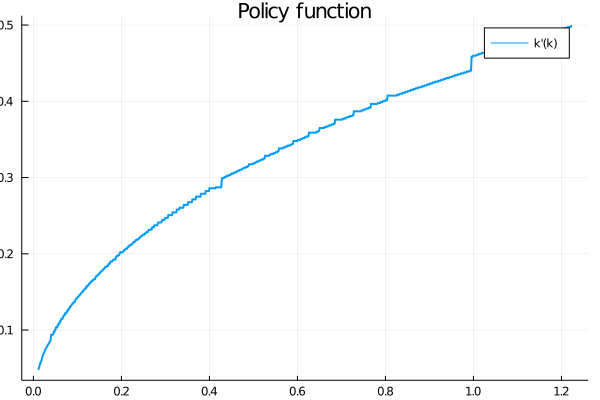
\includegraphics[width=.7\linewidth]{plots/policy.png}
        \caption{Policy function.}
        \label{policy}
    \end{figure}

    \begin{figure}[H]
        \centering
        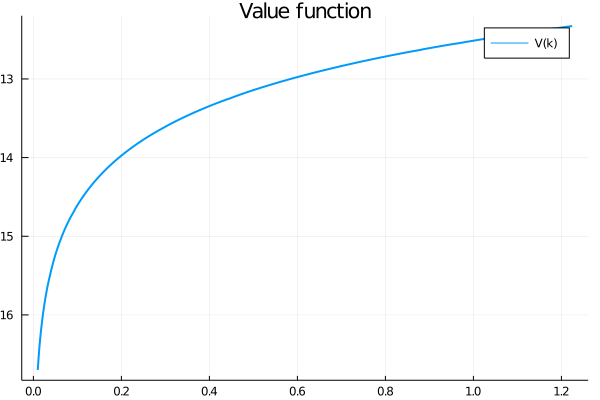
\includegraphics[width=.7\linewidth]{plots/value.png}
        \caption{Value function function.}
        \label{value}
    \end{figure}

\end{homeworkProblem}

\begin{homeworkProblem}

    We start by implementing the shooting algorithm first. This is coded in the transition.jl file, through the function shooting. The function takes the start and end point, together with the function regulating the transition and a series of additional parameters. We use as function for the dynamics the Euler equation of slide 37/68. Starting from the initial level for capital, the function will then guess a new value for the next period and iterate forward the policy function for 200 periods. If at the end of the process the distance with the end point is sufficiently small, the algorithm will stop, otherwise it will guess another second step and start again:

    \begin{verbatim}
    k_path = zeros(steps + 1)
    k_path[1] = k_start

    k_grid = range(max(0, k_start - pert), k_start + pert, length=size_grid)
    print("Searching from $k_start to $k_end, around $k_grid\n")

    for k_t1 in k_grid
        
        k_path[2] = k_t1

        for i in 3:length(k_path)

            k_t2 = fn_k2(k_path[i - 2], k_path[i - 1])

            if k_t2 < 0 break end

            k_path[i] = k_t2 
        end

        if abs(k_path[end] - k_end) < ε
            return k_path
        end
\end{verbatim}

    The shooting function is then actually implemented by the compute\_transition function, which is designed to also incorporate the the inverse shooting method, i.e. guessing capital in the period 200 until, by moving backwards, we find the right initial capital.

    IN carrying on this analysis we need to bear in mind the following caveat. After the productivity shock, in our model it is not given whether the system will have a unique new steady state, as we might have bifurcations depending on the parameter values we choose for the model. In our case, for instance, we try with $\alpha = 0.5$ and $\beta=0.9$ and after the productivity shock ($z=2$), the model has two equilibria, one locally stable at approximately $k'=4$ and one unstable at $k'=0.8$. The system will then immediately converge to the second equilibrium in case the shock pushes capital instantly at the new equilibrium level, but will converge to the first equilibrium or diverge to 0 otherwise. Simply defining the end point as a solution to $k'=\alpha \beta z k^{\alpha}$ is therefore not always correct and a more complex analysis is required.

    The resulting transition path is reported in Figure 3. We can see that the transition takes actually less than 200 periods and capital quickly converges to the new higher steady state.

    \begin{figure}[H]
        \centering
        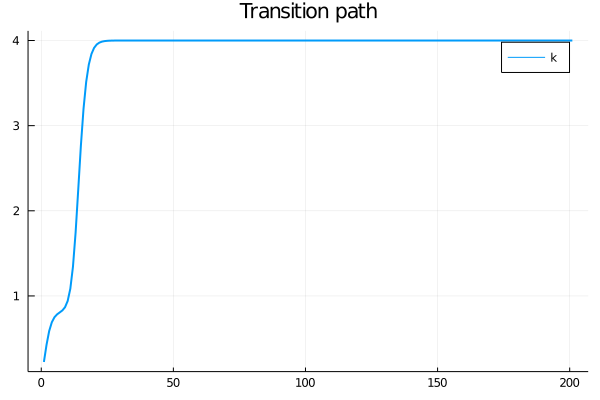
\includegraphics[width=.7\linewidth]{plots/transition_shooting.png}
        \caption{Transition path between two equilibria after productivity shock, according to shooting algorithm.}
        \label{transiiton_shooting}
    \end{figure}

    We give an attempt to solving the system of 200 equations in the system function in transition.jl, but at the moment the solver algorithm cannot find a realistic path for capital (see Figure 4).
    We also try the backward shooting algorithm in the compute\_transition  function, exploiting the same shooting algorithm but with an inverse function for the transition dynamics.
    Unfortunately, in this case the algorithm cannot reach the right starting point for capital, but diverges to 0 (see Figure 5).

    \begin{figure}[H]
        \centering
        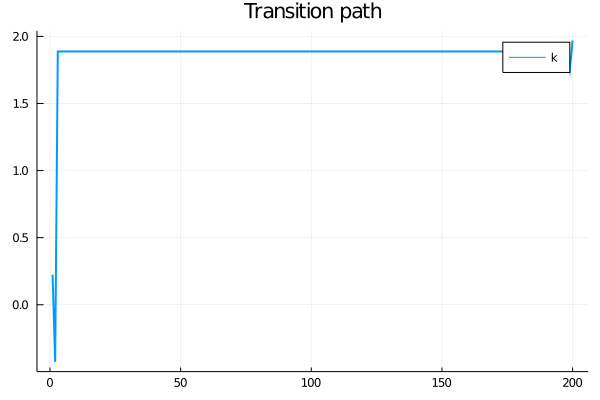
\includegraphics[width=.7\linewidth]{plots/transition_system.png}
        \caption{Transition path between two equilibria after productivity shock according to system algorithm.}
        \label{system}
    \end{figure}

    \begin{figure}[H]
        \centering
        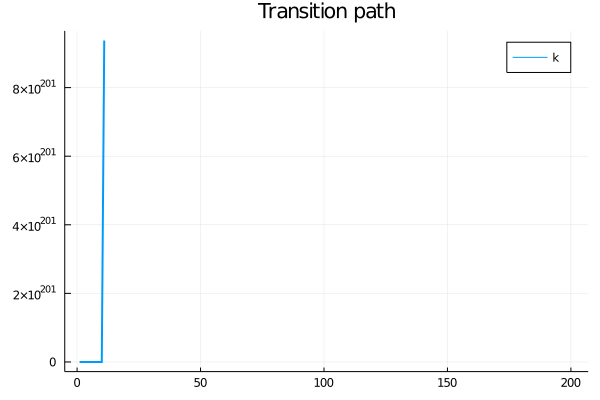
\includegraphics[width=.7\linewidth]{plots/transition_inverse shooting.png}
        \caption{Transition path between two equilibria after productivity shock according to inverse shooting algorithm.}
        \label{inverse_shooting}
    \end{figure}


\end{homeworkProblem}

\begin{homeworkProblem}[4]
    Let $c_n = \frac{b_n - a_n}{2}$ be the middle point in the $i$-th iteration of the bisection method. Now consider the absolute error. By construction in needs to be bounded above by the
    i-th splitting of the interval, hence,

    \begin{equation}
        \abs{c_n - c} \leq \frac{\abs{b - a}}{2^n}
    \end{equation}

    where $c$ is the root of the function $f$. It is straight forward to see then that  $\abs{c_n - c} \xrightarrow{} 0$ linearly at rate $0.5$.

\end{homeworkProblem}

\pagebreak

\nocite{*}
\bibliographystyle{apacite}
\bibliography{bib}


\end{document}